\documentclass[aspectratio=169,11pt]{beamer}
\usetheme{default}
\usefonttheme{professionalfonts}
\usepackage{amsmath,amssymb,graphicx}
\setbeamertemplate{navigation symbols}{}
\setbeamertemplate{footline}[frame number]
\setbeamerfont{frametitle}{series=\bfseries}
\setbeamercolor{frametitle}{fg=black}
\definecolor{acc}{HTML}{1F5FAD}
\setbeamercolor{itemize item}{fg=acc}
\setbeamercolor{enumerate item}{fg=acc}
\newcommand{\hl}[1]{\textcolor{acc}{\textbf{#1}}}

\begin{document}

\begin{frame}{Method: misspecified models \& core code}
\begin{columns}[T]
\begin{column}{0.47\textwidth}
\footnotesize
\hl{Setup (Sec.~IV).} True DGP: $P$ signals, $c=P/T$. We see the first $P_1$, $q=P_1/P$; model complexity $cq$.

\smallskip
\hl{Prop.~6} (ridgeless, $\Psi=\psi I$):
\[\mathcal{E}(0;cq;q)=b_*\psi\min\{q,\,c^{-1}\}\]
flat for $cq>1$: approximation gain $=$ min-norm bias.

\smallskip
\hl{Theorem 1.} With optimal $z_*$: $SR$, $R^2$ strictly increasing \& concave in $q$.\\ Double ascent $\to$ permanent ascent.

\smallskip
\hl{Core module} (\texttt{voc\_core.py}):
\begin{itemize}
\item RFF: $[\sin(\gamma\omega'G),\cos(\gamma\omega'G)]$, $\omega\sim N(0,I)$, $\gamma=2$
\item $\hat\beta=S'(zT\,I_T+SS')^{-1}R$; $z=0$ $\Rightarrow$ pseudo-inverse
\item $P=12{,}000$, 7 $z$, 1{,}079 windows: $\approx1$\,s
\end{itemize}
\end{column}
\begin{column}{0.52\textwidth}
\centering
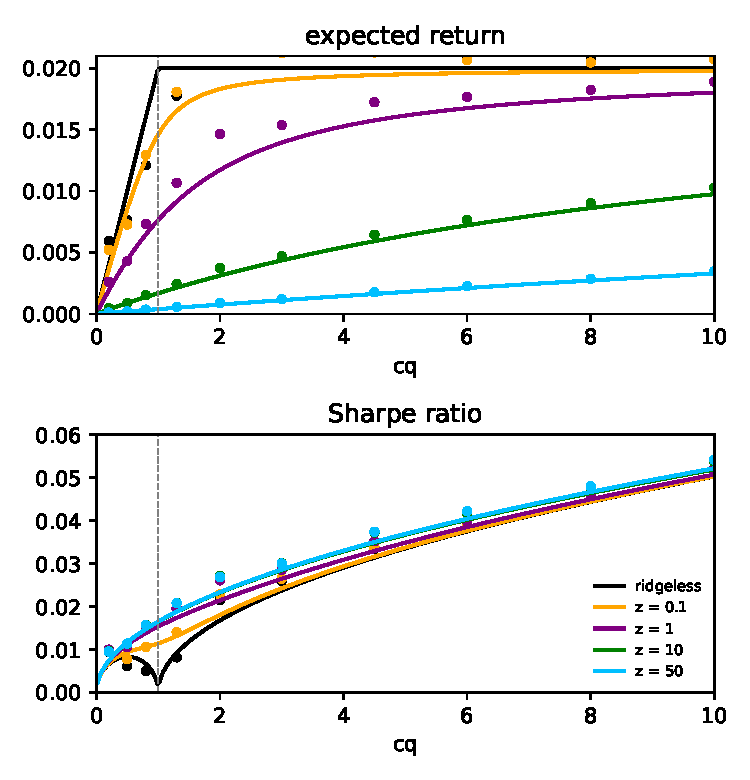
\includegraphics[height=0.72\textheight]{fig_slide_E_SR.pdf}\\
{\scriptsize $\Psi=I$, $b_*=0.2$, $c=10$. Lines: closed form (Prop.~5); dots: Monte Carlo, $T=200$, 20 sims. Cf.\ Figs.~5--6.}
\end{column}
\end{columns}
\end{frame}

\begin{frame}{Next steps}
\begin{enumerate}
\setlength{\itemsep}{7pt}
\item \hl{Real data:} Goyal--Welch predictors $G_t$ (15) $\to$ \texttt{rff()} $\to$ rolling ridge
\item \hl{Backtest (Figs.~7--8):} $T=12$, $P$ up to $12{,}000$, $\log_{10}z\in\{-3,\dots,3\}$\\
10--30 seeds instead of the paper's 1{,}000, reported openly
\item \hl{Table I, linear rows:} same engine with $P=15$; ridgeless via pseudo-inverse
\item \hl{Robustness:} $T\in\{60,120\}$, $\gamma\in\{0.5,1\}$
\item \hl{Critique check:} at $T=12$ with persistent predictors the model is close to\\
time-series momentum (authors, p.~499)
\end{enumerate}
\end{frame}

\end{document}
